\section*{Knowledge Checks}

\subsection*{Connectionless Transport: UDP}
    \subsubsection*{UDP header files}
    \noindent Which fields are in a UDP segment header?
    Source port, destination port, length (of UDP header plus payload), internet checksum

    \subsubsection*{UDP segment length field}
    \noindent Why is the UDP header length field needed?
    Because the payload section can be of variable length, and this lets UDP know where the
    segment ends
    
    \subsubsection*{Internet Checksum and UDP}
    \noindent Over what set of bytes is the checksum field in the UDP header computed over?
    The entire UDP segment, except the checksum field itself, and the IP senders and receive
    address fields
    \begin{itemize}
        \item On the sending side, the UDP sender will take each application-layer chunk of data written into a UDP
        socket and send it in a distinct UDP datagram. And then on the receiving side, UDP will deliver a segment's
        payload into the appropiate socket, preserving the application-defined message boundary.
    \end{itemize}

    \subsubsection*{What is checksum?}
    \noindent The next statements are true about a checksum:
    \begin{itemize}
        \item A checksum is computed at a sender by considering each byte within a packet
        as a number, and then adding these numbers (each number representing a bytes)
        together to compute a sum (which is known as a checksum)
        \item The sender-computed checksum value is often included in a checksum field
        within a packet header
        \item The receiver of a packet with a checksum field will add up the received
        bytes, just as the sender did, and compare this locally-computed checksum with the
        checksum value in the packet header. If these two values are \textbf{different}
        then the receiver \textbf{knows} that one of the bits in the received packet has been changed
        during transmission from sender to receiver.
    \end{itemize}

    \subsubsection*{Computing the internet Checksum (1)}
    \noindent Compute the Internet checksum for these two 16-bit words: 11110101 11010011 and 10110011 01000100
    To compute the Internet checksum of a set of 16-bit words, we compute the one's complement sum 
    of the two words. That is, we add the two numbers together, making sure that any carry into the 17th bit
    of this initial sum is added back into the 1's place of the resulting sum); we then take the one's
    complement of the result. This means that the Internet checksum is \textbf{01010110 11100111}

    \subsubsection*{Computing the internet Checksum (2)}
    \noindent Compute the Internet checksum for these two 16-bit words: 01000001 11000100 and 00100000 00101011
    To compute the Internet checksum of a set of 16-bit words, we compute the one's complement sum 
    of the two words. That is, we add the two numbers together, making sure that any carry into the 17th bit
    of this initial sum is added back into the 1's place of the resulting sum); we then take the one's
    complement of the result. This means that the Internet checksum is \textbf{10011110 00010000}

    \url*{https://traductordebinario.com/calculadora-de-sumas-binario/}
    \linebreak
    \url*{https://www.allmath.com/es/calculadora-del-complemento-a-uno.php}
        

    \subsubsection*{UDP Checksum: how good is it?}
    \noindent When computing the Internet checksum for two numbers, a single flipped bit (i.e., in just one of
    the two numbers) will always result in a changed checksum

    \subsubsection*{UDP Checksum: how good is it?}
    \noindent When computing the Internet checksum for two numbers, a single flipped bit (i.e., in just one of
    the two numbers) will NOT result in a changed checksum.

    \subsubsection*{IP addresses and port numbers in a UDP segment sent in reply}
    \noindent Now consider the UDP datagram (and the IP datagram that will encapsulate it) sent in reply by the
    application on host 128.119.40.186  to the original sender host, labeled B in the figure above.
    \begin{figure}[H]
        \centering
        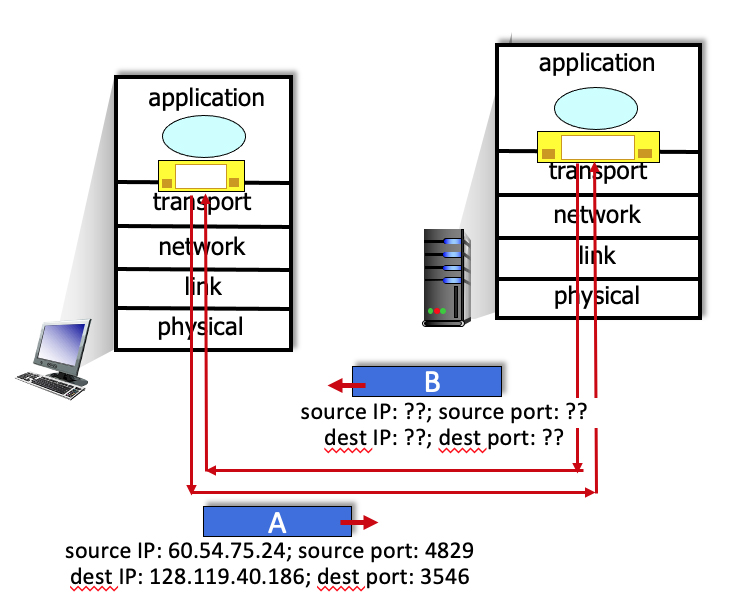
\includegraphics[width=0.5\textwidth]{img/3.3.9.jpg}
        \label{fig:UDP}
    \end{figure}
    \begin{itemize}
        \item The source port number of the UDP segment (B) sent in reply is: \textbf{3546}
        \item The source IP address of the IP datagram containing the UDP segment (B) sent in reply is: \textbf{128.119.40.186}
        \item The destination port number of the UDP segment (B) sent in reply  is: \textbf{4829}
        \item The destination IP address of the IP datagram containing the UDP segment (B) sent in reply is: \textbf{60.54.75.24}
    \end{itemize}

\newpage
\subsection*{Principles of Reliable Data Transfer}
    \subsubsection*{Reliable data transfer protocol mechanisms}
    \noindent Consider the purpose/goals/use of different reliable data transfer protocol mechanism. For the given
    purpose/goal/use this is the RDT mechanism that is used to implement the given purpose/goal/use
    \begin{itemize}
        \item[NAK] Lets the sender know that a packet was NOT received correctly at the receiver
        \item[Checksum] Used by the sender or receiver to detect bits flipped during a packet's transmission
        \item[Sequence numbers] Allows for duplicate detection at receiver
        \item[ACK] Lets the sender know that a packet was received correctly at the receiver  
        \item[Retransmission] Allows the receiver to eventually receive a packet that was corrupted or lost in an
        earlier transmission
    \end{itemize}

    \subsubsection*{Cumulative ACK}
    \noindent What is meant by cumulative acknowledgment, ACK(\textit{n})?
    A cumulative ACK(\textit{n}) acks all packets with a sequence number up to and including \textit{n} as being received

    \subsubsection*{Stop-and-wait: channel utilization}
    \noindent Suppose a packet is 10k bits long, the channel transmission rate connecting a sender and receiver is
    10 Mbps, and the round-trip propagation delay is 10 ms. What is the maximum channel utilization of a stop-and-wait
    protocol for this channel?
    \[U_{sender}=\frac{L/R}{RTT+L/R}=\frac{10,000/10,000,000}{0.01+10,000/10,000,000}=0.09\approx0.1\]
    where
    \begin{itemize}
        \item[L] packet size 
        \item[R] transmission rate
        \item[RTT]  Round-trip propagation
    \end{itemize}

    \newpage
    \subsubsection*{Channel utilization with pipelining}
    \noindent Suppose a packet is 10K bits long, the channel transmission rate connecting a sender and receiver is
    10 Mbps, and the round-trip propagation delay is 10 ms. What is the channel utilization if a pipelined protocol
    with an arbitrarily high level of pipelining for this channel?
    \[U_{sender}=\frac{N*L/R}{RTT+L/R}\]
    where
    \begin{itemize}
        \item[L] packet size 
        \item[R] transmission rate
        \item[RTT]  Round-trip propagation
        \item[N] packet pipelining increased utilization 
    \end{itemize}

    \subsubsection*{Channel utilization with pipelining (more)}
    \noindent Suppose a packet is 10K bits long, the channel transmission rate connecting a sender and receiver is
    10 Mbps, and the round-trip propagation delay is 10 ms. How many packets can the sender transmit before it starts
    receiving acknowledgment back?
    The answer is 10 packets

    \subsubsection*{Pipelining}
    \noindent The next statements are true about pipelining:
    \begin{itemize}
        \item A pipelined sender can have trasmitted multiple packets for which the sender has yet to receive an ACK from the
        receiver
        \item With a pipelined sender, there may be transmitted packet "in flight" - propagating through the channel - packets
        that the sender has sent but that the receiver has not yet received
    \end{itemize}

    \subsubsection*{Packet buffering in Go-Back-N}
    \noindent What are some reasons for discarding received-but-out-of-sequence packets at the receiver in GBN?
    \begin{itemize}
        \item The sender will resedn that packet in any case
        \item The implementation at the receiver is simpler
    \end{itemize}

    \subsubsection*{Packet buffering in Go-Back-N (more)}
    \noindent What are some reasons for \textit{not} discarding received-but-out-of-sequence packets at the receiver in GBN?
    \begin{itemize}
        \item Even though that packet will be retransmitted, its next retransmission could be corrupted, so don't discard
        a perfectly well-received packet
    \end{itemize}

    \subsubsection*{Receiver operation in Selective Repeat}
    \noindent In the SR receiver window (see diagram below), why haven't the red packets been delivered yet?
    \begin{figure}[H]
        \centering
        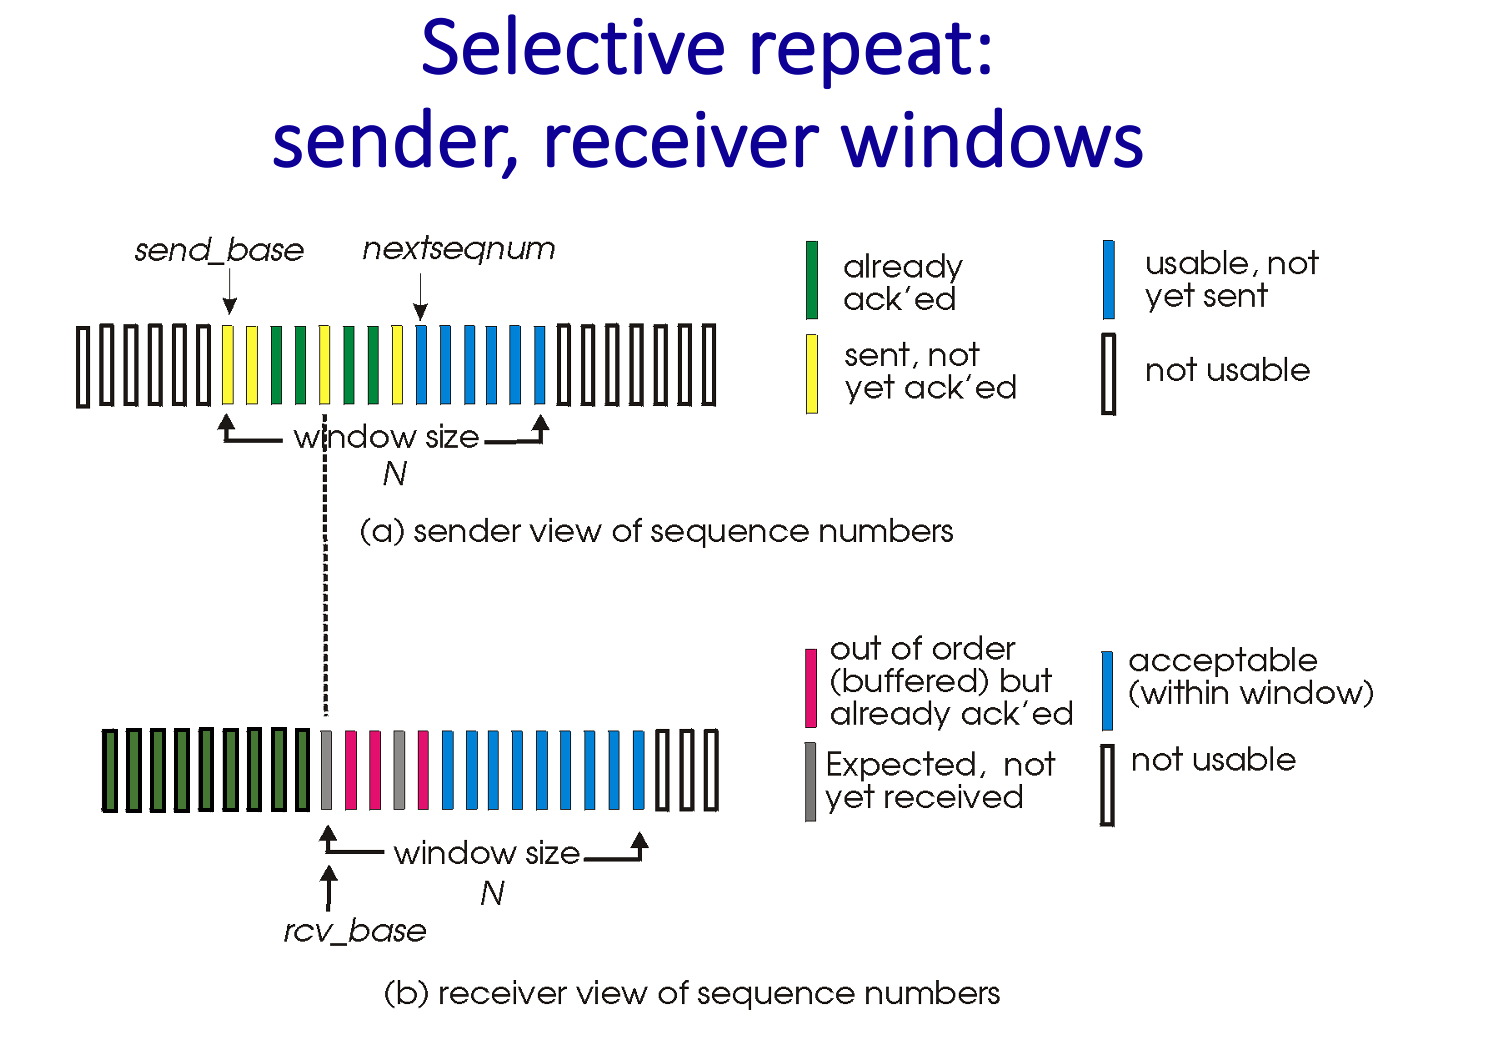
\includegraphics[width=0.5\textwidth]{img/3.4.13.jpg}
    \end{figure}
    There is a packet with a lower sequence number than any of the red packets that has yet to be received, so in-order dalivery
    of data in the red packets up to the application layer is not possible

    \subsubsection*{Receiver operation in Selective Repeat (more)}
    \noindent In SR, why does the receiver have to acknowledge packets with sequence numbers that are less than those in its 
    window, which starts at \textit{rcv-base}
    \begin{figure}[H]
        \centering
        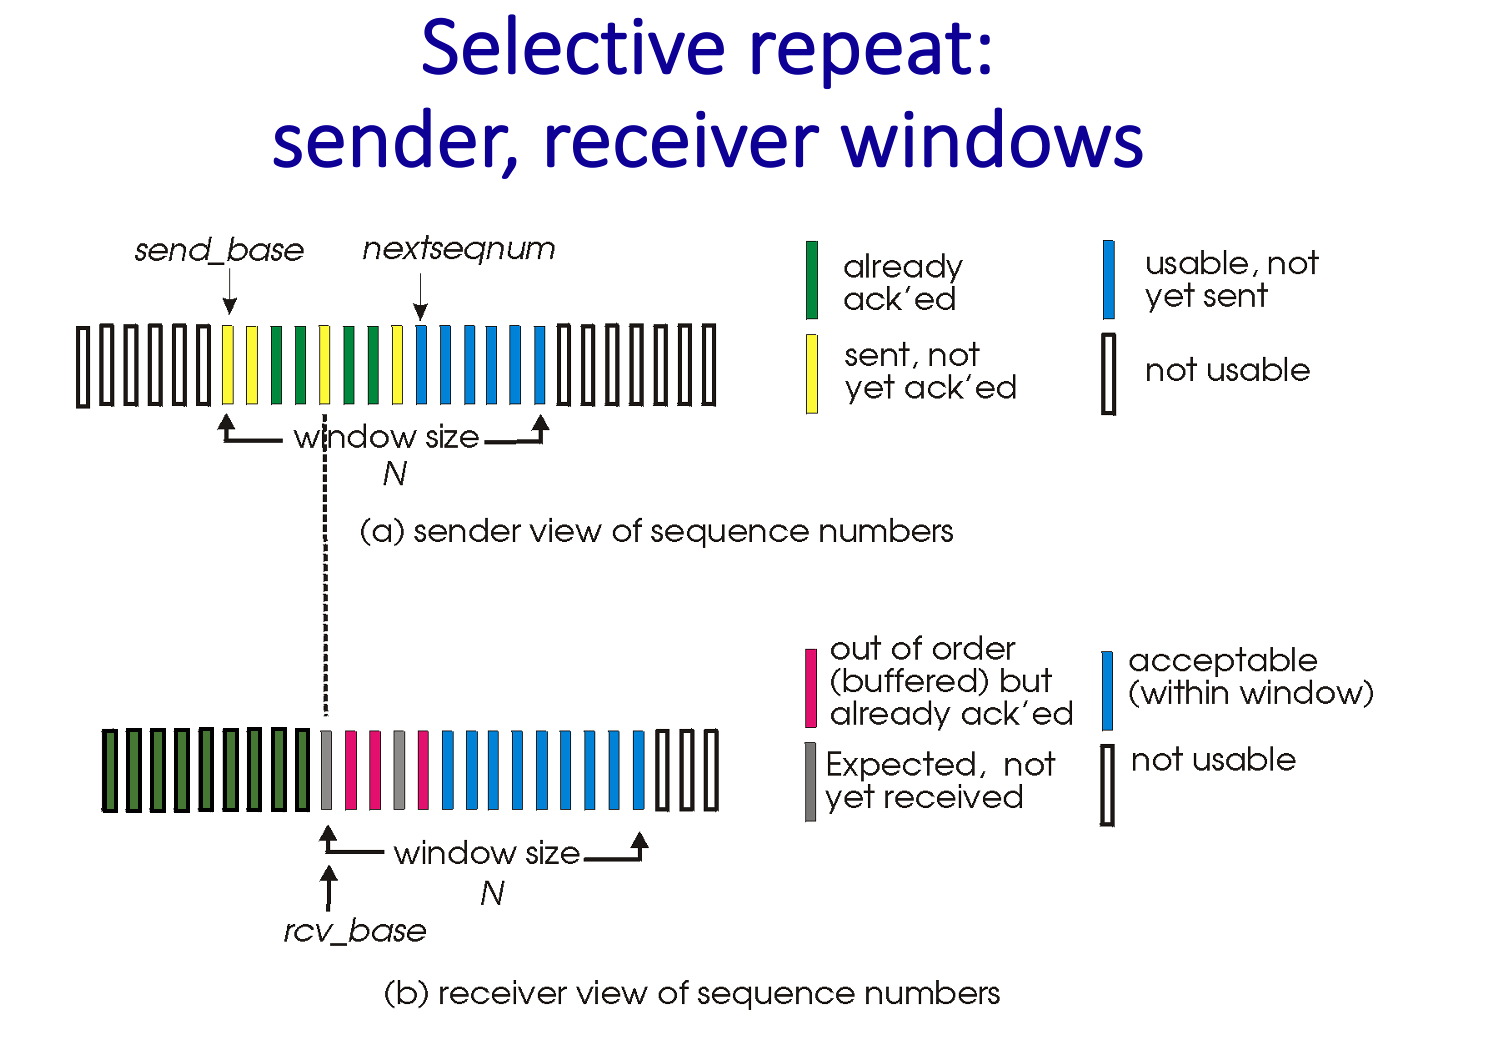
\includegraphics[width=0.5\textwidth]{img/3.4.13.jpg}
    \end{figure}
    Because the sender may not have received an ACK for that packet yet

\subsection*{Connection-oriented Transport: TCP}
    \subsubsection*{Reliable data transfer protocol mechanisms}
    \subsubsection*{Cumulative ACK}
    \subsubsection*{Stop-and-wait: channel utilization}
    \subsubsection*{Channel utilization with pipelining}
    \subsubsection*{Channel utilization with pipelining (more)}
    \subsubsection*{Pipelining}
    \subsubsection*{Packet buffering in Go-Back-N}
    \subsubsection*{Packet buffering in Go-Back-N (more)}
    \subsubsection*{Receiver operation in Selective Repeat}
    \subsubsection*{Receiver operation in Selective Repeat (more)}

\subsection*{Principles of Congestion Control}
    \subsubsection*{Congestion control versus flow control}
    \subsubsection*{Two congested senders}
    \subsubsection*{Different approaches towards congestion control}

\subsection*{TCP Congestion Control}
    \subsubsection*{TCPs AIMD algorithm}
    \subsubsection*{TCPs AIMD algorithm (2)}
    \subsubsection*{TCPs Slowstart algorithm}